\documentclass[a4,12pt]{article}
\usepackage[T1]{fontenc}
\usepackage{epigraph}
\usepackage{textcomp}
\usepackage[utf8]{inputenc}
\usepackage[english]{babel}
\usepackage{graphics}
\usepackage{graphicx}
\usepackage{epstopdf}
\usepackage{amsmath}
\usepackage{hyperref}
\usepackage{fancyvrb}
\usepackage{verbatim}
\usepackage{cmap}
%\renewcommand{\familydefault}{\sfdefault}
\textwidth=16cm
\oddsidemargin=0.1cm
\linespread{1.2}

\title{KernelGen -- multi-target accelerated kernels\linebreak generator for Fortran programs}
\author{Dmitry N. Mikushin\\ maemarcus@gmail.com}

\newcommand{\HRule}{\rule{\linewidth}{0.5mm}}
\DefineVerbatimEnvironment{code}{Verbatim}{frame=single, fontsize=\small}

\begin{document}

\maketitle

\begin{abstract}

KernelGen is open source-to-source translator with Fortran frontend, multiple backends (currently CUDA, OpenCL and CPU) and common runtime library. Fortran frontend extracts computational loops out of original source code, replacing them with calls to equivalent GPU or APU kernels. Additionally frontend can generate functions for per-kernel automatic results comparison between different implementations of the same loop. Runtime library handles both static (modules data, global variables) and dynamic (variables, fixed shape or allocatable arrays) kernel dependencies, automatically performing data load into device memory and fetching back the results. Runtime is designed thread-safe to provide seamless multi-GPU support for multithread and MPI applications. This article includes both simple test case for demonstration and real application study. To become production-ready prototype a couple of important device code optimization techniques must be implemented in KernelGen: tiling for shared memory utilization and loops interchanging.

\end{abstract}

\pagebreak

\setlength{\epigraphwidth}{8cm}
\epigraph{Those that can, do. Those that can't, complain.}{Torvalds, Linus}

\section{Motivation}

During last 5 years GPGPU technologies became wide-spread. Although mature programming models exist as well as publicly available compilation toolkits, most of applications ported to GPUs (considering real ones, not highly-tuned benchmarks) are rather simple or utilize GPU computations only for small subsets of code. There is a number of reasons behind this situation:

\begin{enumerate}
\item In complex applications it is often impossible to identify and port a single compute-intensive block of code, as soon as computations are distributed between multiple major units. For example in case of WRF or COSMO weather prediction models time of single block typically never exceeds ~10-15\% of total time. Thus, single block port cannot deliver impressive overall speedup. Still, choosing a well-localized block with minimum external dependencies is the only way to accomplish GPU port and present results shortly.
\item Consider the application block is ported. Then how to integrate it to the usual application development process, if core team has no much knowledge in GPU computations? How much support it would take to keep block updated? Without integration port becomes a branched case study.
\end{enumerate}

This effort is dedicated to implementing hybrid CPU-GPGPU extendable Fortran compiler that can fully conserve original CPU source code, and therefore minimize implicit complications in user-side development process. Fully automatic compilation should not be confused with various existing directive-based approaches (PGI, HMPP), that still require too much hand-coding.

\section{Strategy}

No doubt, developing toolchain for automatic GPU kernels generation is a very complex long-term task. To move forward step-wise, the problem could be represented as a number of ring passes. On the first round we would need a rough mechanism for identifying computational loops and moving them into separate functions (host-device code split). Second, there should be a rough generator translating Fortran code into representation, that could be chained to existing GPU code compilers. Next we need previously implemented loop identification tool to insert calls to special runtime library functions that would invoke kernels and pass their data dependencies between host and device memories. During passed rounds a set of behavior tests should be collected for regressions checks. Next important group of rounds are optimizations. Toolchain needs to provide an approach for applying kernel code analysis and recompilation in runtime, taking in account additional information like actual compute grids sizes. With this mechanism implemented, a round of optimization passes development can start. According to known practices, the most important optimizations should be loops interchanging and tiling for threads and shared memory utilization. For better code coverage several specific limitations also need to be relaxed, such as inlining external calls in GPU kernels. At this point complete functional prototype will be created, and development could switch back onto improving rough base components.

KernelGen, the compilation toolchain being developed, follows above plan and currently reached the step of implementing optimization passes. It means the tool already ports simple loops pretty well and can handle a large subsets of real source codes, falling back to host compiler in places where rough host-device split fails.

\section{Code generator}

The whole host and device code generation process is depicted on Fig.~\ref{fig:pipeline}. Note it covers only static pipeline, where device code is compiled in binary form. KernelGen currently also implements embedding kernel code IR for further compilation and optimization in runtime.

\begin{figure}
\centering
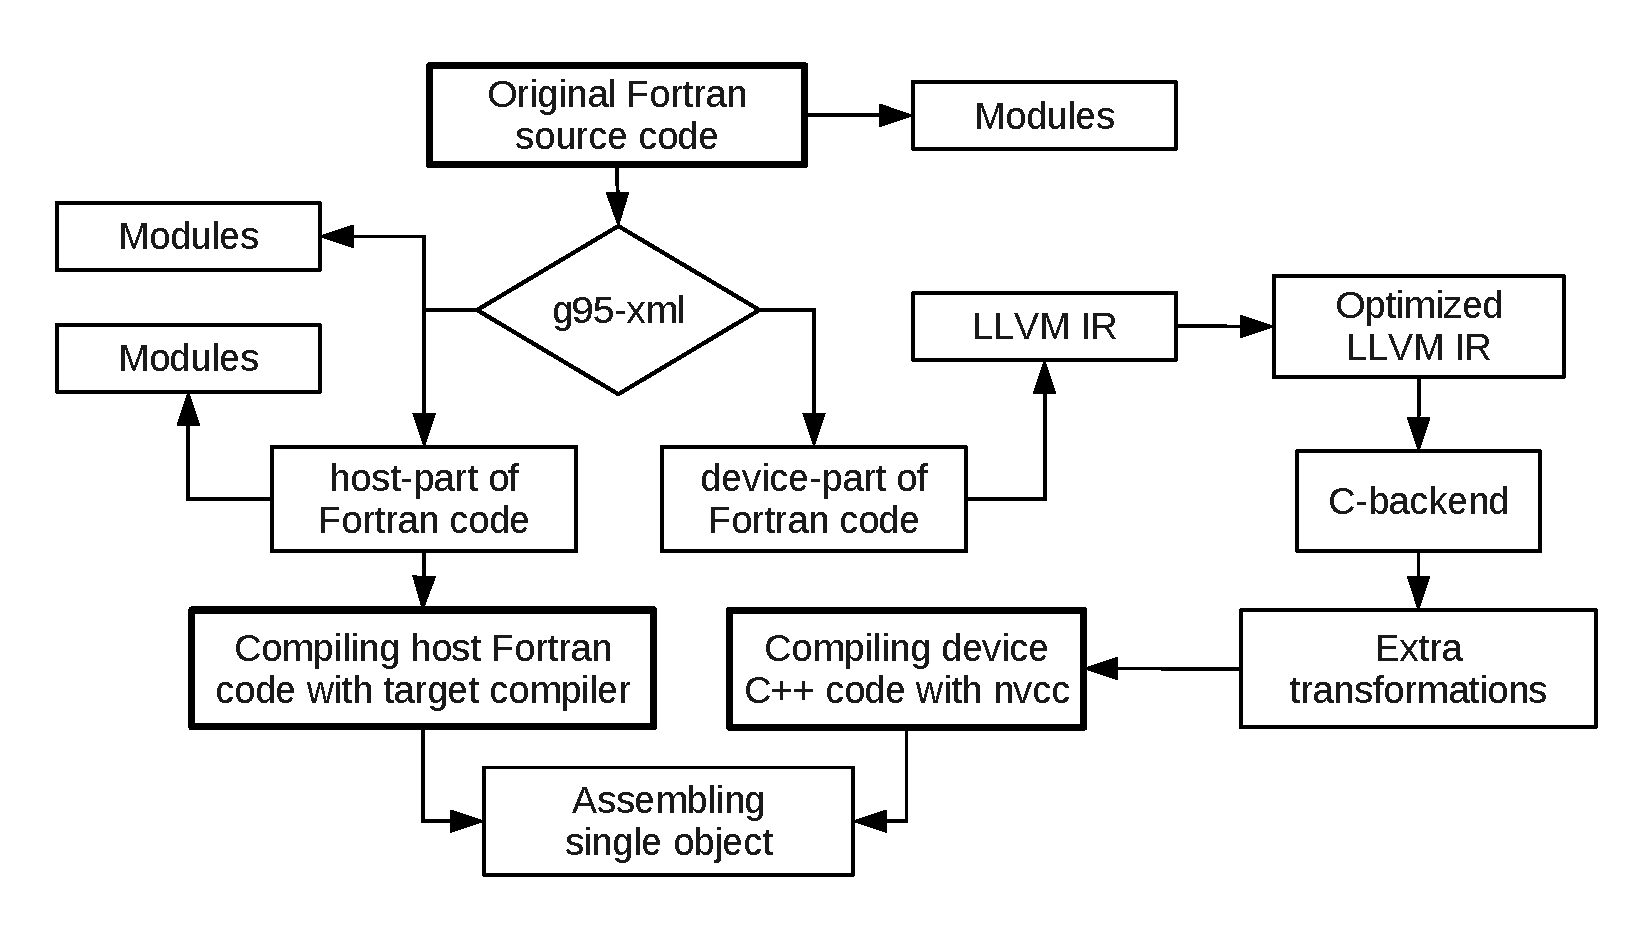
\includegraphics[scale=0.5]{figures/pipeline.pdf}
\caption{KernelGen static code generation pipeline}
\label{fig:pipeline}
\end{figure}

\subsection{Kernels selection}

To identify compute kernels and move them into separate compilation units, Fortran source code is marked up with XML into pretty-printed AST and transformed to target representation using a set of XSL transformations. XML markup is performed using g95-xml, a tool written by Philippe Marguinaud based on g95 compiler parser. Surprisingly, XSLT suited very well for fast development of rough implementation, thanks to its functional nature and builtin tree flow. However, XSL language is not very human-readable, processing is quite slow on huge compilation units and suffers from various fails, such as g95 language support issues or unhandled program logic cases in XSLT. The tool is known to provide good support for Fortran 90/95 and some features of Fortran 2003, like inline functions.

It is planned XML-based parser on some further step will likely be replaced by direct kernels generation out of LLVM IR. Although, currently it is not clear how to set up a split point with LLVM in a way that host code would still be Fortran, in order to utilize external Fortran compilers, other than LLVM over DragonEgg.

\subsection{Backend}

The kernel selection step provides host and device code as output, both in Fortran. Free compilers from standard Fortran to GPU assembly do not exist, although there is good progress in generating PTX assembly and OpenCL code from LLVM IR. Still, while direct IR code generators for CUDA and OpenCL are too incomplete, the LLVM C backend was patched to work as device code generator:

$$
Fortran~code\xrightarrow{dragonegg}LLVM~IR\xrightarrow{C~backend}CUDA~or~OpenCL\xrightarrow{compiler}device~code
$$

\subsection{Runtime vs compile-time generation}

Device code could be either generated during compile time or postponed for runtime. During compile time certain problems cannot be solved, like inlining kernels dependencies, and optimization capabilities are limited. Currently KernelGen generates kernels binaries at compile time and embeds them into executable image together with original IR code, that could be used for runtime recompilation.

\subsection{Bitness}

As soon as the generated device code data is transparently shared with host and most OpenCL devices are 32-bit, in case of OpenCL backend current implementation is limited to 32-bit support. It should be possible to convert structured bitness-dependent data on-the-fly, but it's a complex task, and known practices should be studied first. Relaxing this limitation is very important.

\section{Runtime library}

KernelGen runtime library is a background layer organizing interaction between host and device code. The whole execution process is depicted on Fig~\ref{fig:execution}. Currently runtime implements the following calls:

\begin{itemize}
\item \emph{set\_device} -- select device platform and ID to execute entire host thread kernels on
\item \emph{launch} -- launch device kernel with a given compute grid ranges and data dependencies. This call is inserted in places of original host loops ported to GPUs.
\item \emph{parse\_args/parse\_deps} -- parse the kernel data dependencies and represent them with a set of non-overlapping memory regions.
\item \emph{map/unmap} -- share the set of data dependencies with the specified pointers, sizes and Fortran array descriptors between host and device either by zero-copy access or explicit copying.
\item \emph{build} -- build kernel in runtime from LLVM IR or OpenCL binary.
\item \emph{compare} -- compare results of kernel execution and its equivalent host implementation.
\end{itemize}

\begin{figure}
\centering
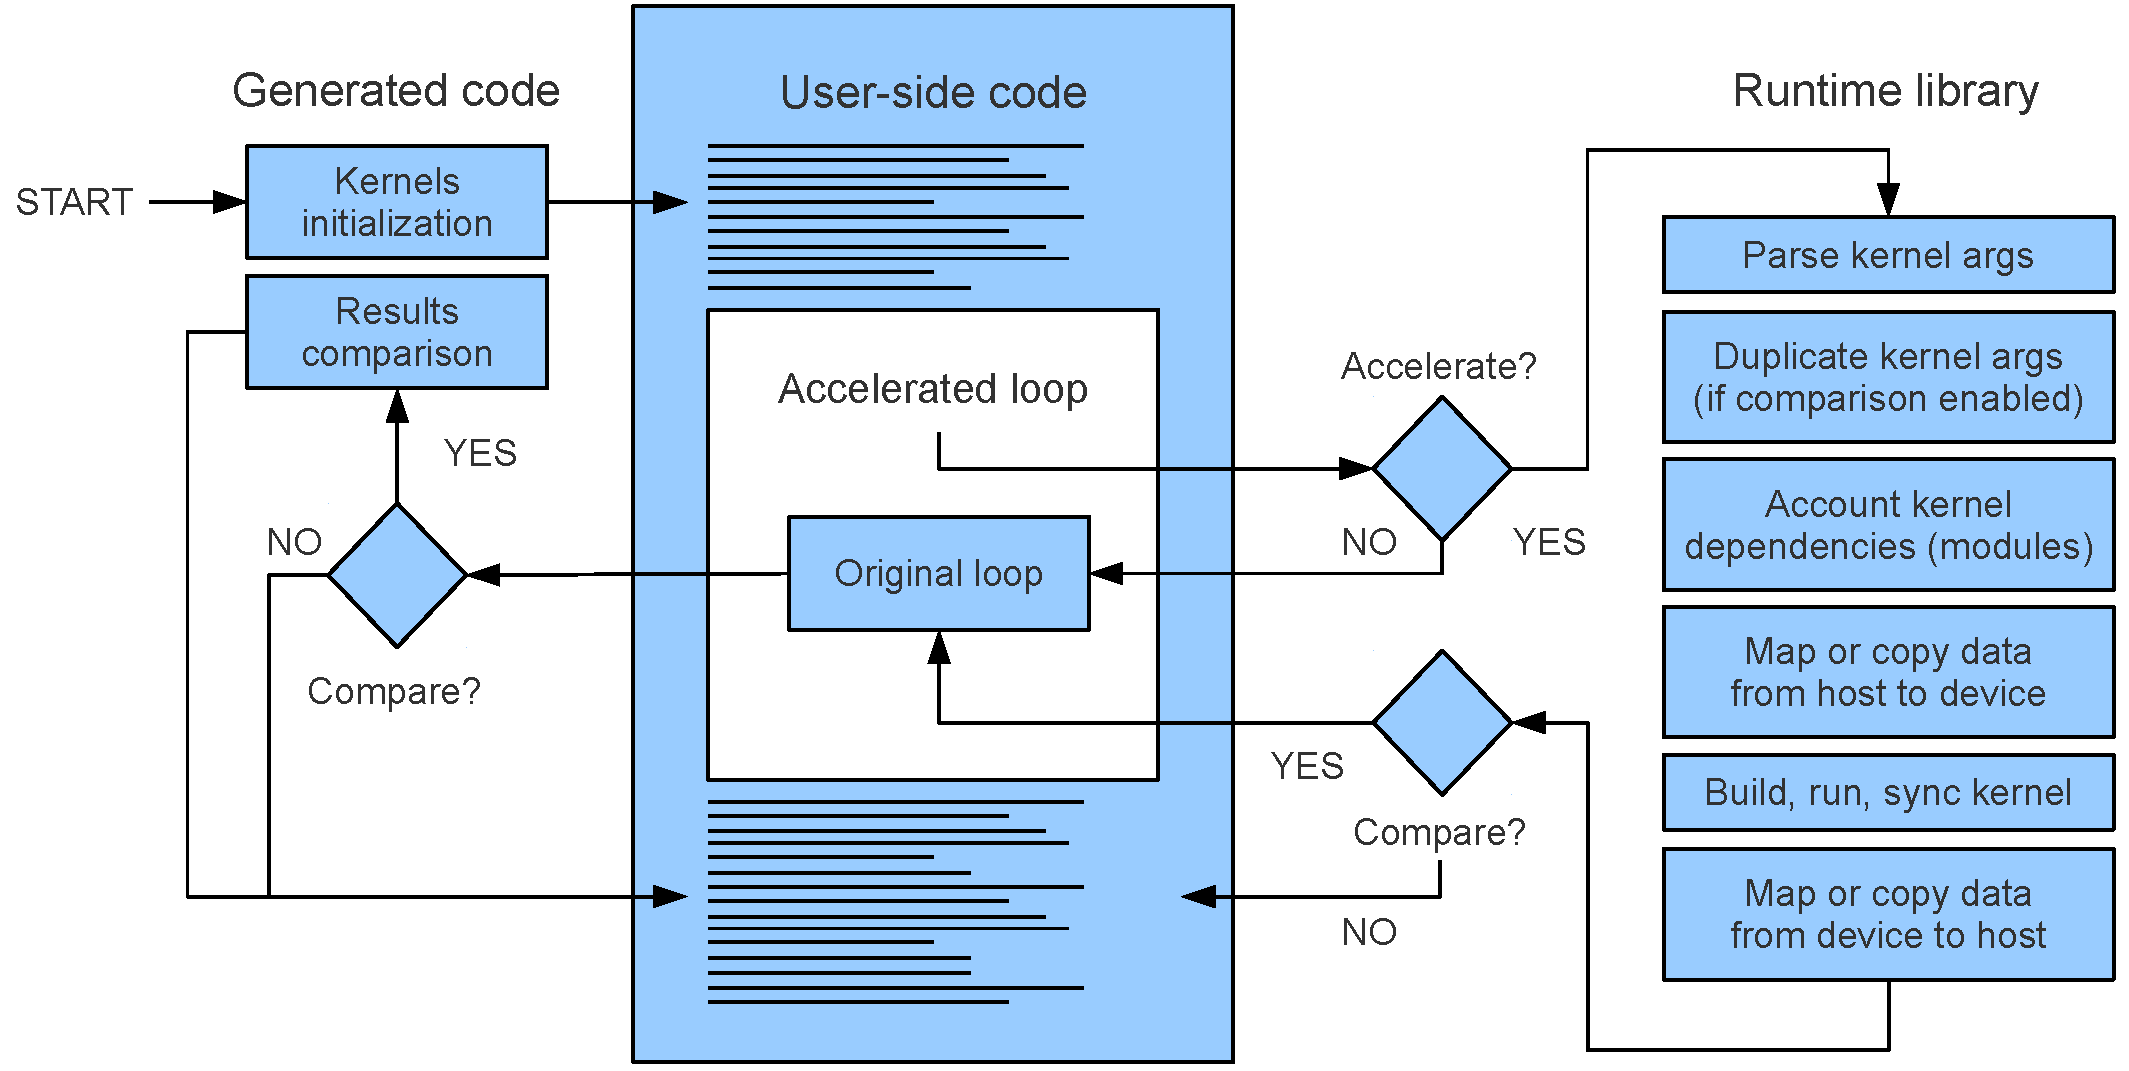
\includegraphics[scale=0.4]{figures/execution.pdf}
\caption{Execution model}
\label{fig:execution}
\end{figure}

\subsection{Multithreading and MPI support}

To track current status and configuration properties, each kernel needs a unique handle. In multithreaded applications such handle must be also unique for each thread running entire kernel and be kept in thread local storage, as soon as different threads may utilize different devices with specific parameters. KernelGen runtime API provides a \emph{set\_device} call to assign specific devices to application threads or processes.

\subsection{Results comparison}

In complex software it's hard to perform accurate results comparison due to various noise - differences in compilers, order of operations, etc. Moreover, on long scales model trajectories tend to deviate too much to distinguish error from natural chaos. To overcome these effects, KernelGen includes a special subsystem for micro-scale testing. For each kernel a special routine performing input and output data comparison can be automatically generated. If difference exceeds the specified fixed value, kernel will be marked as erroneous and fallback to CPU implementation.

\section{Examples}

Consider the following plain Fortran subroutine:

\begin{code}
subroutine sincos(nx, ny, nz, x, y, xy)
implicit none
integer, intent(in) :: nx, ny, nz
real, intent(in) :: x(nx, ny, nz), y(nx, ny, nz)
real, intent(inout) :: xy(nx, ny, nz)
integer :: i, j, k
do k = 1, nz
  do j = 1, ny
    do i = 1, nx
      xy(i, j, k) = sin(x(i, j, k)) + cos(y(i, j, k))
    enddo
  enddo
enddo
end subroutine sincos
\end{code}

KernelGen is capable to translate it to CUDA or OpenCL kernel. Fig.~\ref{fig:sincos_perf} shows the performance of this test on $512\times 512\times 64$ grid on various hardware. AMD E-350 uses AMD APP SDK 2.5, NVIDIA Tesla -- CUDA 4.0. More specific language constructs are also supported: allocatable arrays, derived types and modules.

\begin{figure}
\centering
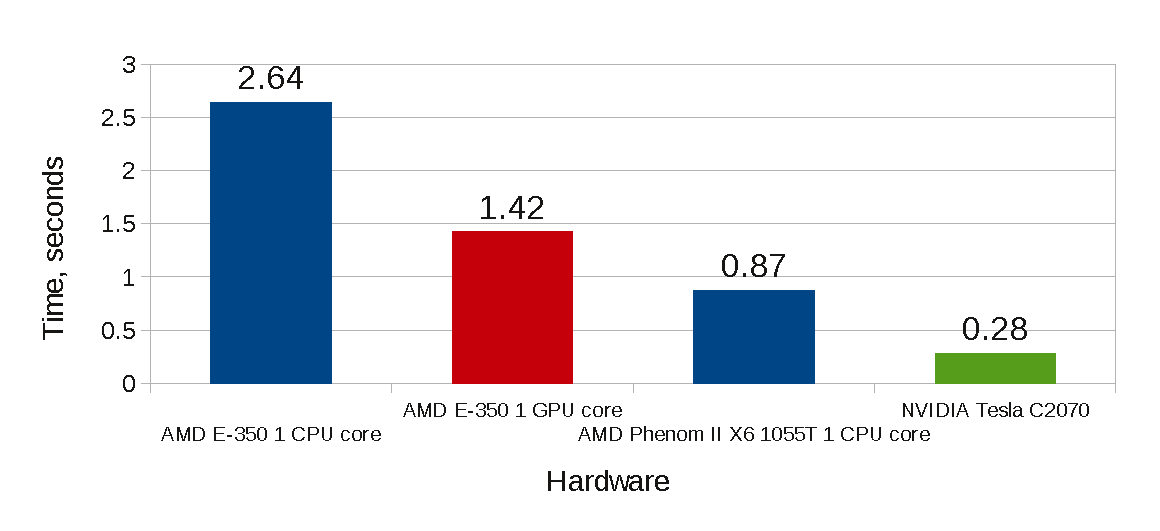
\includegraphics[scale=0.8]{figures/sincos.pdf}
\caption{Performance of sincos kernel generated by KernelGen on AMD and NVIDIA GPUs compared to 1 CPU core.}
\label{fig:sincos_perf}
\end{figure}

Above test is more for simple illustration. KernelGen can handle much more complicated computational software. For 250,000 lines of COSMO regional weather prediction model it generates 1,901 kernels. Not all kernels can give performance benefit, it should be noted once again KernelGen misses several important optimization techniques for tiling and loops interchanging. Still, on Tesla it is already able to beat single 1055T core, showing up to 1.3x speedup on certain kernels.

\section{Conclusions}

Preliminary implementation of GPU kernels generator out of Fortran source code has been developed. Even without important optimizations, it is already able to show speedups against CPU cores on GPUs from the corresponding classes of systems. Real test cases has been studied, current runtime library is stable enough to operate thousands of kernels.

\section{Resources}

Project source code is hosted on hpcforge.org. To fetch the most recent version, checkout the svn repository (as of 29 Aug 2011 9 AM EST the newest one was r414):

\begin{code}
svn checkout
  svn://scm.hpcforge.org/var/lib/gforge/chroot/scmrepos/svn/kernelgen
\end{code}

Another option is to download and install prebuilt rpm binaries found on the project main page:
\begin{code}
https://hpcforge.org/projects/kernelgen/
\end{code}

To build from source code, use instructions listed at 
\begin{code}
https://hpcforge.org/plugins/mediawiki/wiki/kernelgen/index.php/Compiling
\end{code}

Project source code includes behavior and performance tests, to build them follow steps listed at 
\begin{code}
https://hpcforge.org/plugins/mediawiki/wiki/kernelgen/index.php/Testing.
\end{code}
By default make scripts should build both CUDA and OpenCL tests for 32-bit mode and only CUDA for 64-bit mode. Add compiler option \emph{\-Wk,\-\-keep} to keep intermediate files with extracted kernel, IR and device code in the current directory.

\section{Acknowledgments}

This work is a deep fusion of open-source software, business opportunities and scientific customers interests. With support and good will of Dr Gdaly Rivin and Dr Vladimir Krupchatnikov (Roshydromet, Russian Met Office) it became possible to start analyzing the needs of state-of-art weather forecasting models and focus on tool specifically for scientific development. Also with great support of various communities it became possible to reach the present state from ground level with minimum resources just in 5 months. I'd like to thank Roshydromet fellows Artem Petrov for coordination, testing and development, Dr Yulia Martynova for testing KernelGen with WRF model. I'm grateful to Sergey Kovylov of NVIDIA for constant support, Philippe Marguinaud of Meteo France for discussions and bug fixes in g95xml, Alexander Myltsev for testing and polishing build process, LLVM developers and specially Duncan Sands for discussions and bug fixes in C backend, GFortran team and specially Dr Tobias Burnus for Fortran consults and suggestions, Polly/LLVM team and specially Tobias Grosser for intensive discussions on optimizations related to polyhedral analysis. Thanks to Christopher Bergström of Pathscale for discussions and criticism.

\end{document}
